% !TEX root = ../../main.tex


\begin{figure}[!htb]
\vspace{10mm}
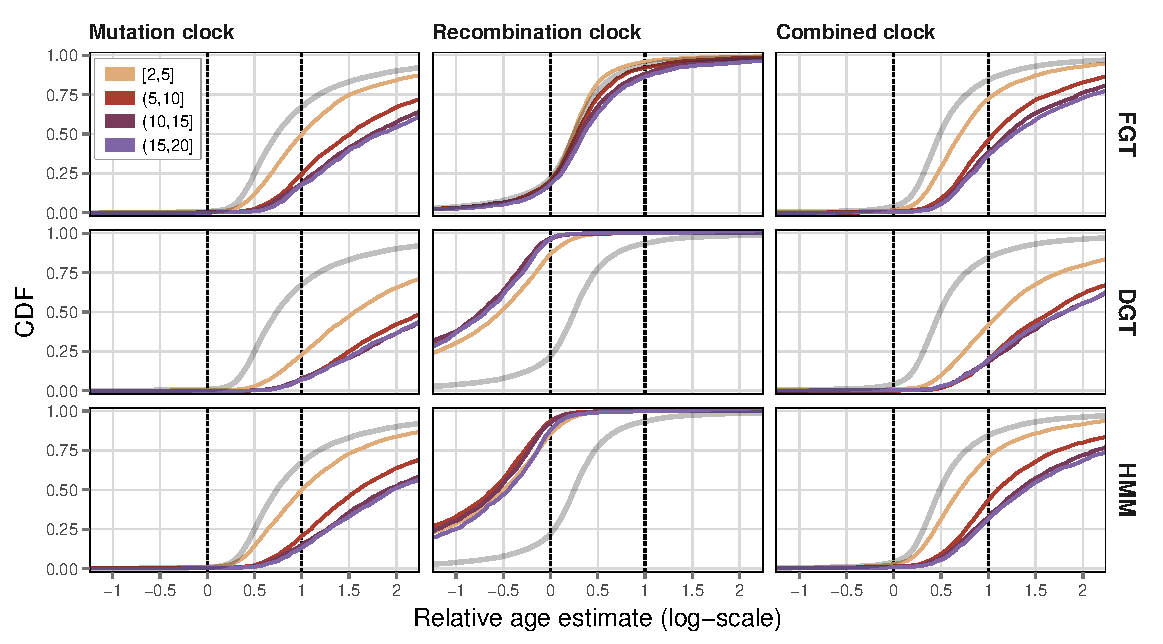
\includegraphics[width=\textwidth]{./img/ch5/vanilla_hist}
\Caption{Relative age using different IBD detection methods}
{The \n{3} IBD detection methods implemented in \texttt{rvage} were compared, \ie \gls{fgt}, \gls{dgt}, and \gls{hmm} (indicated at the \emph{right} of each row), under each clock model (indicated at the \emph{top} of each column).
The relative age, ${\hat{t}_\textit{rel}}$, was calculated as given in \cref{eq:age_relative}, such that $t_c$ and $t_d$ sit at 0~and~1 (\emph{dashed} lines).
The \gls{cdf} of relative age estimates is shown for different frequency ranges; namely \fk{[2,5]}, \fk{(5,10]}, \fk{(10,15]}, and \fk{(15,20]}.
The \emph{grey} line provides a comparison to age estimated using true IBD information as shown in \cpref{fig:discords_hist}, but for \fk{[2,20]}.}
{fig:vanilla_hist}
\end{figure}
